\documentclass[preprint,numbers,10pt]{sigplanconf}

\usepackage{hyperref}
\usepackage{graphicx}
\usepackage{xcolor}
\newcommand\comment[1]{\textcolor{blue}{#1}}

\begin{document}

\title{Language Workbench Challenge 2016: the JetBrains MetaProgramming System}

\authorinfo{Eugen Schindler}{}{eugenschindler@gmail.com}
\authorinfo{Klemens Schindler}{}{klemensschindler@gmail.com}
\authorinfo{Federico Tomassetti}{Independent}{federico@tomassetti.me}
\authorinfo{Markus V\"{o}elter}{}{voelter@gmail.com}
\authorinfo{Kolja Dummann}{}{k.dummann@gmail.com}
\authorinfo{Remi Bosman}{}{remi.bosman@gmail.com}
\authorinfo{Ana Maria \c{S}ut\^{i}i}{}{farcasia@gmail.com}

\maketitle

%%%%%%%%%%%%%%%%%%%%%%%%%%%%%%%%%%%%%%%%%%%%%%%%%%%%%%%%%%%%%%%%%%%%%%%%%%%%%%%
%
% Introduction
%
%%%%%%%%%%%%%%%%%%%%%%%%%%%%%%%%%%%%%%%%%%%%%%%%%%%%%%%%%%%%%%%%%%%%%%%%%%%%%%%

\section{Introduction}

In this paper, we are going to discuss how the JetBrains MetaProgramming System can be used to address the problems presented in the Language Workbench Challenge 2016 (LWC'16).

The JetBrains MetaProgramming System (MPS) is a mature Language Workbench based on projectional editing. While other Language Workbenches are based on projectional editing (the Whole Platform \cite{solmi2005whole}, MetaEdit+ \cite{Tolvanen2006}, Intentional Domain Workbench \cite{Simonyi2006}) MPS is arguably the most mature, with a growing user base.

We believe that one key feature to make MPS successful is its flexibility. By using a powerful and flexible Language Workbench such MPS we, as Language Engineers, can provide languages and corresponding tools that support a significant overhaul of the processes of an organization. It is frequently the case that such processes involve very different kinds of users with very different backgrounds, experiences, and needs. Therefore a complete solution could potentially encompass different aspects of the internal processes, providing different views and a variety of tools such as simulators, debuggers, code-generators, and more.

The ability to support different notations, to process models in different ways, to perform validation and support testing: all these features and others are necessary to build solutions as complete as demanded in real-life scenarios.

Considering the comparison of Language Workbenches features presented in \cite{erdweg2015evaluating} we can see that MPS is among the most complete Language Workbenches. Other tools with a comparable level of completeness are \emph{MetaEdit+} and the \emph{Whole Platform}. While \emph{Xtext} \cite{Eysholdt2010} has a strong support in many areas it is strictly confined to the textual notation and this limitation sets it apart from multi-notation Language Workbenches such as MPS.

With respect to the feature model presented in \cite{erdweg2015evaluating} the only features missing in MPS are \emph{Free-form editing} and \emph{Live translation}.

\subsection{JetBrains MPS in previous challenges}

TODO: Summarize results of MPS in previous challenges

\subsection{Problems presented in the LWC'16}

The problems identified for the LWC'16 permit to evaluate very different aspects of a Language Workbench. By addressing all three of them we aim to offer a complete picture of the potentialities (and possibly the limitations) offered by MPS.

The first problem is regarding \textbf{Notation}. By addressing this problem we aim to demonstrate how MPS can support several, very different notations. Notations are particularly relevant because they are the most visible aspect of languages. In many cases, Language Workbenches are used to create Domain Specific Languages. Such languages are intended to appeal a specific category of subjects. This category could be familiar with specific notations, not necessarily textual. Being able to support the notations of preference of the target audience can be a key element to winning users support. 

The second problem considers \textbf{Evolution and Reuse}. These are characteristics which are absolutely crucial for the maintenance of a solution in the long run. Any mature engineering approach should consider the whole lifecycle of the proposed solution. The evolution is particularly important for languages because they are tools used to represent knowledge, probably the most valuable asset for many companies. By being able to evolve languages we can preserve the investment done in building models using those languages. Reuse is another key element because it permits to significantly reduce the cost of developing complex solutions. For example, several projects based on MPS benefit from reusing languages provided as part of the \emph{mbeddr platform} \footnote{See \url{http://mbeddr.com/platform.html}}.

Finally, the third problem is about \textbf{Editing}. This aspect is particularly relevant for projectional editors because they usually require users to part from the traditional textual editing experience. This transition requires significant training and it can be a cause of resistance. By improving the editing experience we can reduce this risk. While the usability of the MPS editors have been previously deemed positive by users \cite{Voelter2014} we believe is still an aspect which needs to be emphasized. By addressing this particular problem we aim to prove the progresses of MPS in this area and highlight possible necessary improvements still needed.

\subsection{Structure of the paper}

In the rest of the paper we are going to present our proposed solutions to the three different problems (\emph{Notation, Evolution and Reuse, and Editing}). For each problem we will start by describing the assumptions, then we will discuss the implementation, separately for each point, and after that we will analyze each problem according to this schema: Variants, Usability, Impact, Composability, Limitations, Uses and examples, Effort (best-effort), Other comments, Artifact.

Finally, we will draw our conclusions.

%%%%%%%%%%%%%%%%%%%%%%%%%%%%%%%%%%%%%%%%%%%%%%%%%%%%%%%%%%%%%%%%%%%%%%%%%%%%%%%
%
% Notation Section
%
%%%%%%%%%%%%%%%%%%%%%%%%%%%%%%%%%%%%%%%%%%%%%%%%%%%%%%%%%%%%%%%%%%%%%%%%%%%%%%%

\section{Addressing the Notation Problem}

\subsection{Assumptions}

\subsection{Implementation}
The implementation for this challenge is located in a repository on github \footnote{https://github.com/mps-lwc-16/mps-lwc-16}. To explore the implementation, please clone the repository and follow the instructions in the README.md.

Many of the challenge items can be demonstrated using examples from the \emph{mbeddr platform} \footnote{See \url{http://mbeddr.com/platform.html}}, so we have used examples from there whenever appropriate.

We have written models in the mbeddr documentation language to present the implementation. To open the documentation model for the implementation to this challenge, open the Notation model, as shown in Figure \ref{fig:opennotation}. The Notation chapter is divided into sections, each of which addresses one or more of the challenge items. Each of those items is discussed in detail in the subsections below.

\begin{figure}[p]
	\centering
	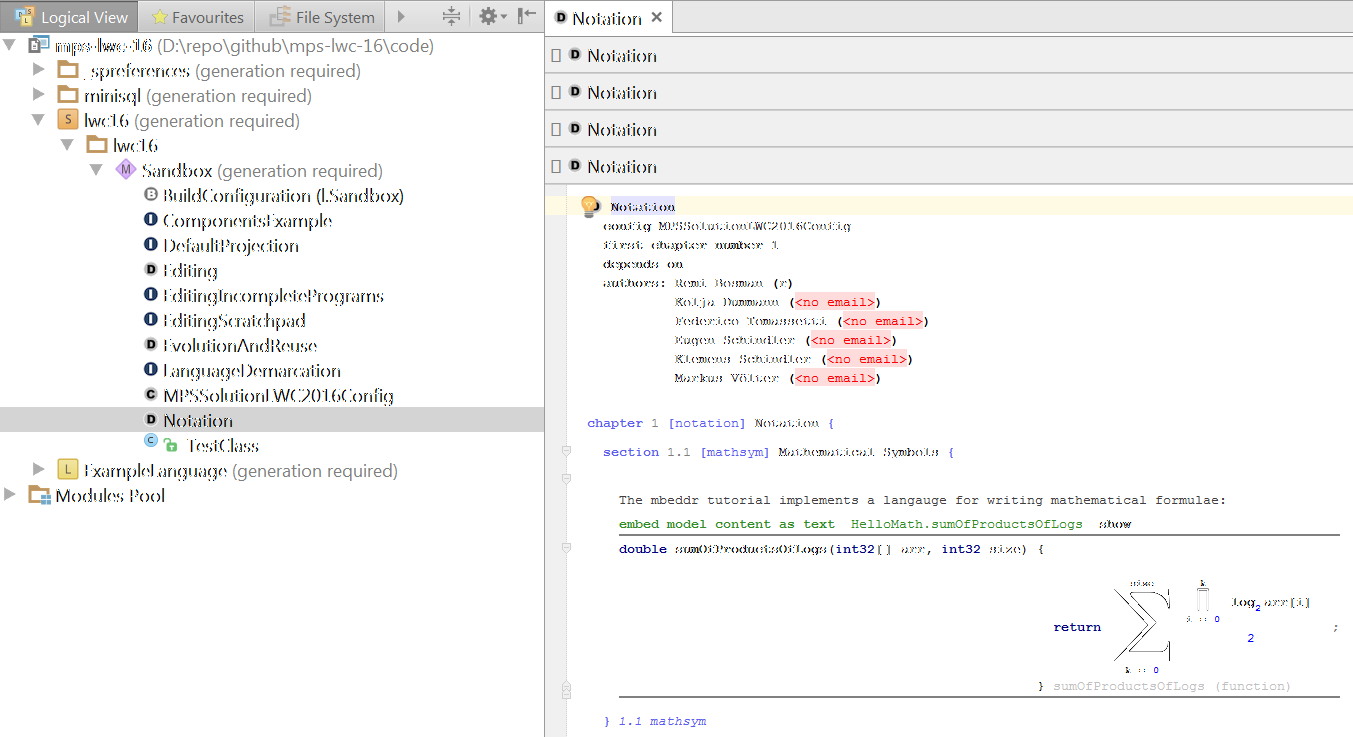
\includegraphics[width=0.50\textwidth]{screens/OpenNotation.png}
	\caption{The documentation model for the Notation challenge}
	\label{fig:opennotation}
\end{figure}

\subsubsection{Support mathematical symbols in addition to textual notation}
Figure \ref{fig:mathnotation} shows a mathematical calculation expressed in the mbeddr math language, which is embedded in a function of the mbeddr C language.
\begin{figure}[p]
	\centering
	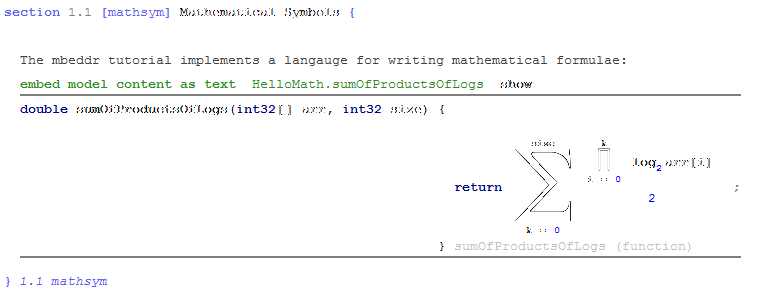
\includegraphics[width=0.50\textwidth]{screens/MathematicalNotation.png}
	\caption{Mathematical notation for the mbeddr math language}
	\label{fig:mathnotation}
\end{figure}

\subsubsection{Support tabular notation in addition to textual notation}\label{sec:tabnot}
Figure \ref{fig:txtnotationsm} shows a textual notation for the mbeddr statemachine language, while Figure \ref{fig:tabnotationsm} shows a tabular notation for the same model expressed in the same statemachine language.
\begin{figure}[p]
	\centering
	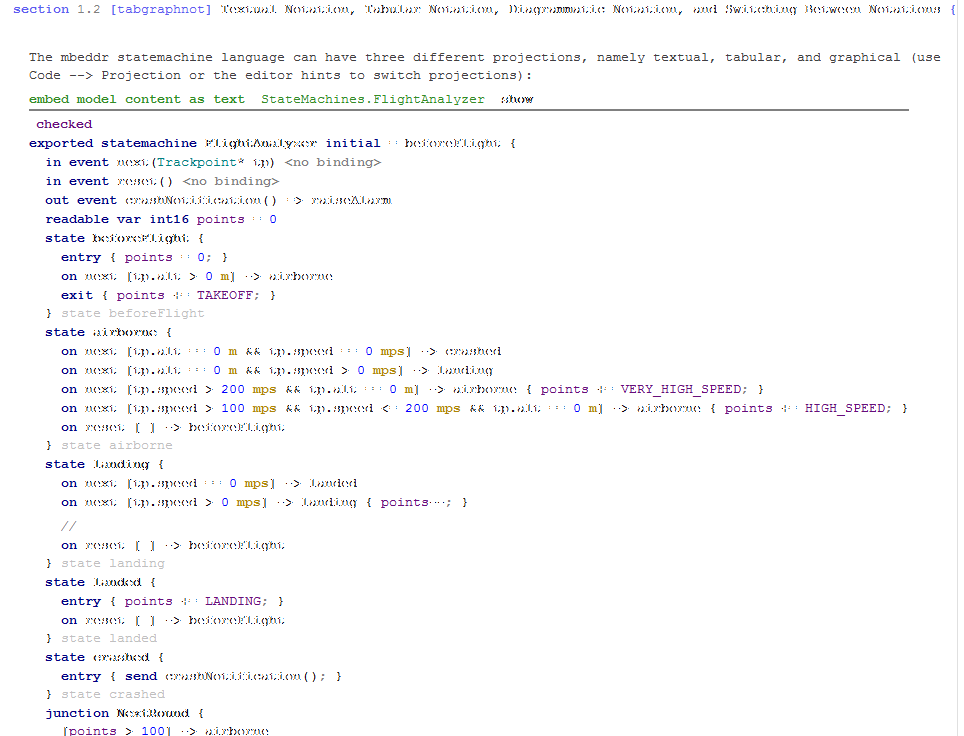
\includegraphics[width=0.50\textwidth]{screens/TextualNotationStatemachine.png}
	\caption{Textual notation for the mbeddr statemachine language}
	\label{fig:txtnotationsm}
\end{figure}

\begin{figure}[p]
	\centering
	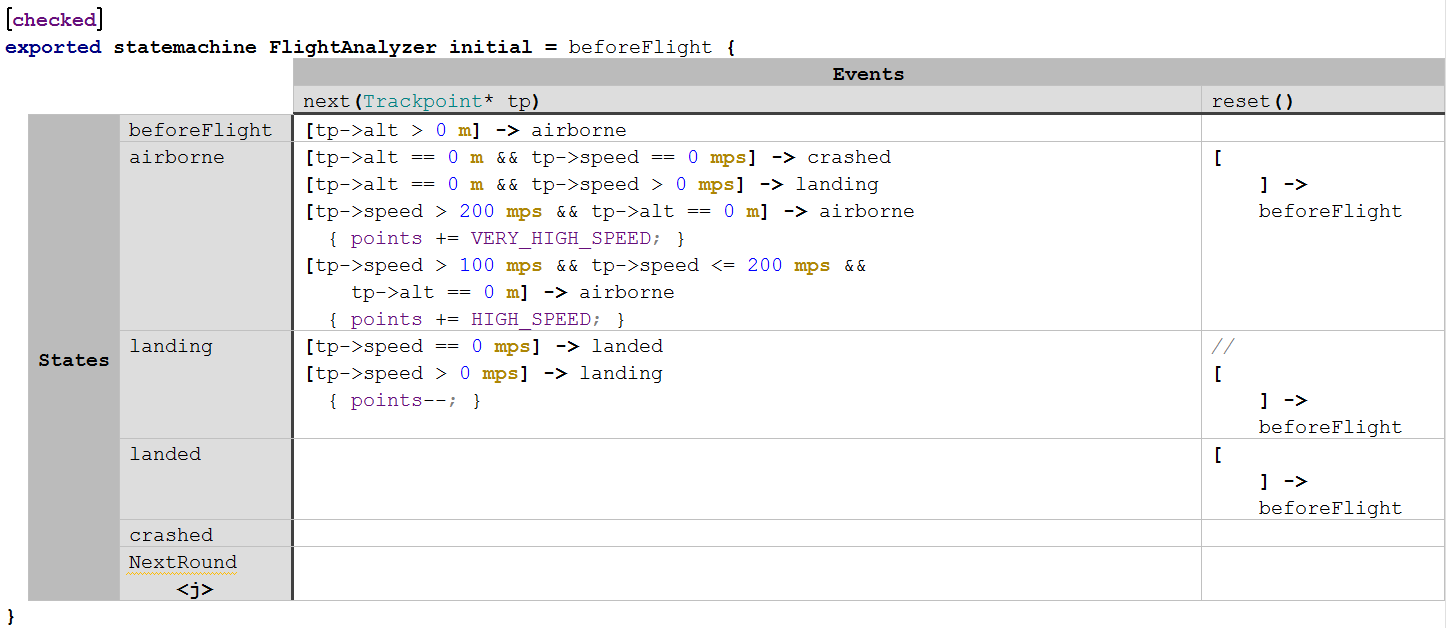
\includegraphics[width=0.50\textwidth]{screens/TabularNotationStatemachines.png}
	\caption{Tabular notation for the mbeddr statemachine language}
	\label{fig:tabnotationsm}
\end{figure}

\subsubsection{Support diagrammatic notation in addition to textual notation}\label{sec:dianot}
Figure \ref{fig:dianotationsm} shows a diagrammatic notation for the mbeddr statemachine language, for exactly the same model as also shown in Section \ref{sec:tabnot}.

\begin{figure}[p]
	\centering
	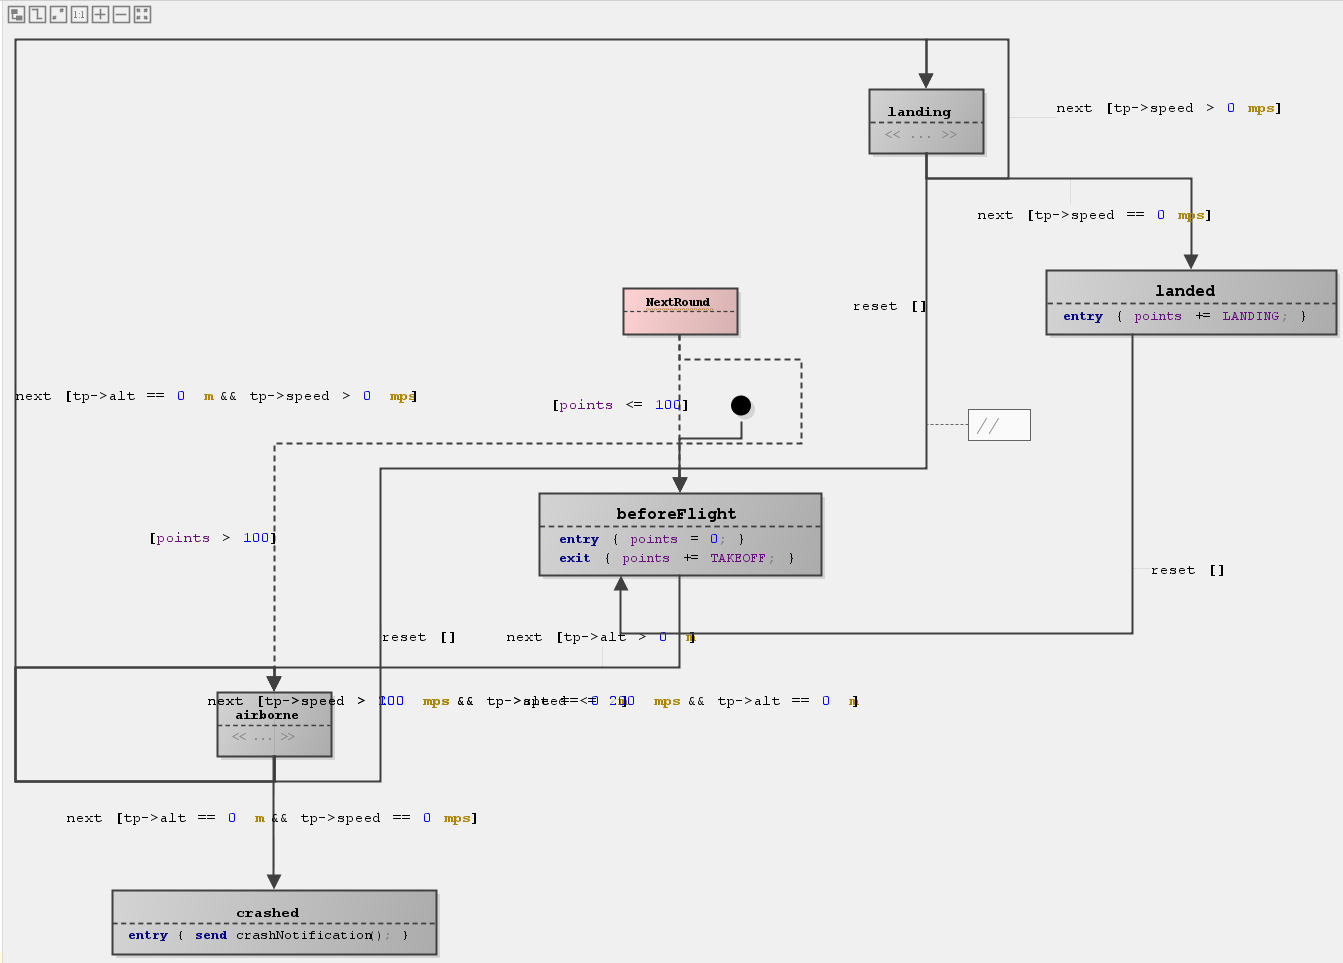
\includegraphics[width=0.50\textwidth]{screens/DiagrammaticNotationStatemachines.png}
	\caption{Diagrammatic notation for the mbeddr statemachine language}
	\label{fig:dianotationsm}
\end{figure}

\subsubsection{Support switching between multiple alternative notations for the same language}
As shown in Sections \ref{sec:tabnot} and \ref{sec:dianot}, the notation for the same model written in the mbeddr statemachine language can be alternated between textual, tabular, and diagrammatic.

\subsubsection{Generic metadata annotations: annotation of program elements without changing their core meaning}
\subsubsection{Optional hiding: hide parts of the code, without losing the content and while retaining editability}
\subsubsection{Computed properties: read only annotations that are automatically derived form the main program}
\subsubsection{Computed structures: structured, editable views}
\subsubsection{Skeleton editing: guide the user with syntactic templates with editable holes}
\subsubsection{Embedding code in prose: mix structured code with free text}
\subsubsection{Embedding blackboxes: allow program elements to be opaque non-textual elements}

\subsection{Variants}

\subsection{Usability}

\subsection{Impact}

\subsection{Composability}

\subsection{Limitations}

\subsection{Uses and examples}

\subsection{Effort (best-effort)}

\subsection{Other comments}

\subsection{Artifact}

%%%%%%%%%%%%%%%%%%%%%%%%%%%%%%%%%%%%%%%%%%%%%%%%%%%%%%%%%%%%%%%%%%%%%%%%%%%%%%%
%
% Evolution and Reuse Section
%
%%%%%%%%%%%%%%%%%%%%%%%%%%%%%%%%%%%%%%%%%%%%%%%%%%%%%%%%%%%%%%%%%%%%%%%%%%%%%%%

\section{Addressing the Evolution and Reuse Problem}

In this section we present our solution to the problem about Evolution and Reuse.

\subsection{Assumptions}

Our solutions are presented making references to the two main language families developed for MPS.

First of all we have the BaseLanguage, which is an implementation of Java built from JetBrains and shipped with MPS. Several extensions are distributed with MPS, including extensions to support lambdas, manipulation of sequences, expressions to access MPS concepts and models, etc.

Another very popular family of languages is mbeddr. It is an implementation of the C language in MPS with support for variability, state machines, testing, documentation and more. In addition to the the mbeddr platform has been created. It is a collection of language extensions not specifically related to mbeddr or the C language. These extensions proved to be useful in were different contexts.

\subsection{Implementation}

In this subsection we present how we implemented a solution to each specific challenge.

\subsubsection{Language extension: modularly extend a language with new syntactic constructs}
\label{evr:langext}

In this section, we are going to describe the mbeddr language for state
machines with event-driven execution. The mbeddr state machines extends
the base language from MPS. This enables a seamless integration between
C code and state machine specifications.

State machines are a mathematical model of computation often used in embedded software
for describing discrete behaviour through state transitions. Its characterizing
ingredients are states, transitions and events. At any given time, a state
machine is in a state and it can be transitioned from one state to another.
A transition in a state machine is triggered by an event. These events
are usually provided by the environment, and, hence, the state machine
needs to have a way to interact with the environment. Besides events,
transitions can also have different guard expressions that need to hold when
the event arrives, for the transitions to be triggered.

We are now going to describe the extension of mbeddr with new syntactic notations for state machines.

In mbeddr, the state machine language is packaged in a language module and it
extends the base language of MPS. The \emph{StateMachine} concept extends
\emph{BaseConcept}, which means that the state machine is a program node,
as \emph{BaseConcept} is the concept from which all other concepts are derived.
The state machine language also implements the \emph{IModuleContent} interface,
which means that they can be top-level components in modules or can be inside of any
container that expects \emph{IModuleContent} children. Modules in mbeddr C
introduce basic program modularization, visibility control and namespaces \cite{voelter2013mbeddr}.

In the next paragraphs, we are going to present excerpts from a state machine for
judging flights. The state machine awards points for successful
takeoff and landing and for speed flown \cite{voelter2014generic}.

The state machine adds custom notation for specifying the state machine. The textual
form of the state machine can be seen in Figure \ref{fig:HFAT}. The figure depicts a hierarchical state machine
that computes the points for a flight.
In addition, because textual forms can live alongside graphical and tabular forms in MPS, 
the state machine can be viewed in table form and graphical form as well alongside the piece of C code
where it is used. Figure \ref{fig:HFATab} shows the same state machine for flight analyzes in tabular form.

\begin{figure}[ht!]
	\centering
	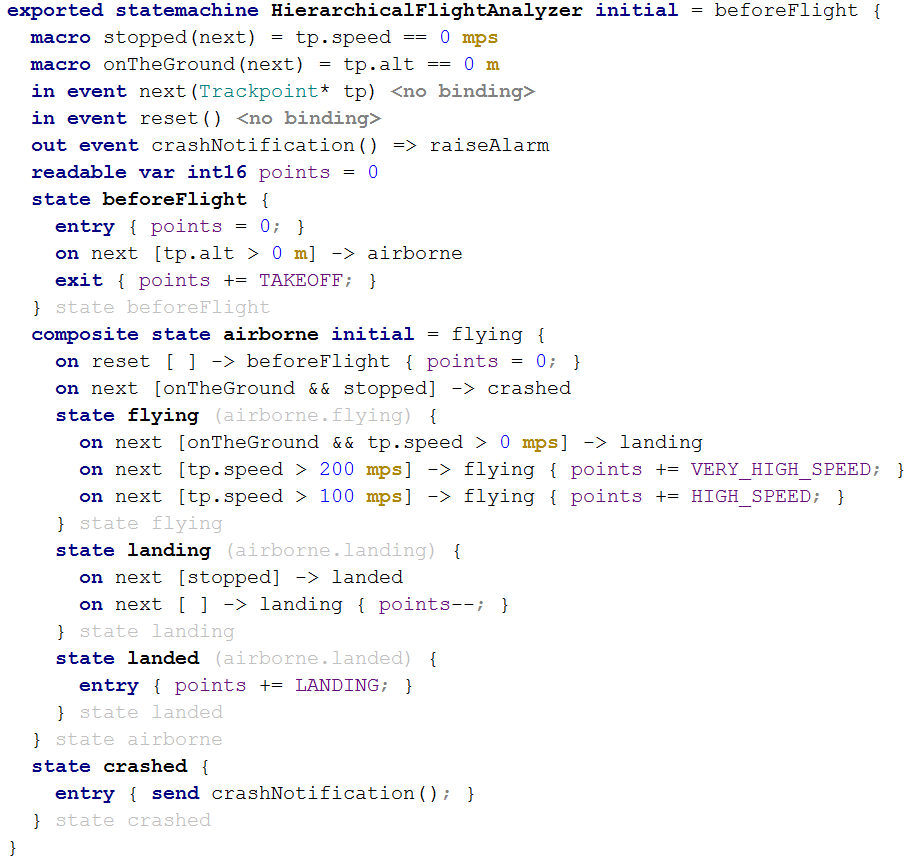
\includegraphics[scale=0.5]{screens/HierarchicalFlightAnalyzerT}
	\caption{Hierarchical flight analyzer state machine - textual notation}
	\label{fig:HFAT}
\end{figure}

\begin{figure*}[ht!]
	\centering
	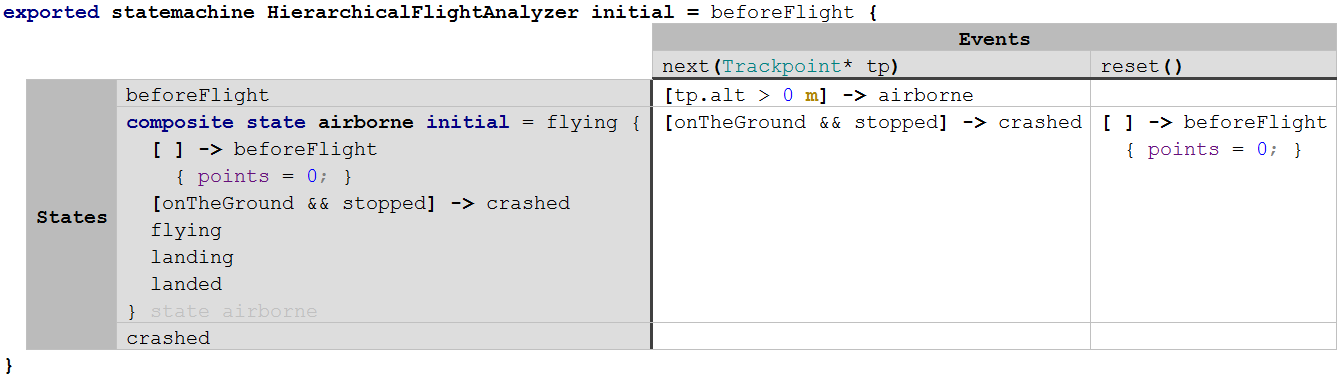
\includegraphics[scale=0.55]{screens/HierarchicalFlightAnalyzerTab}
	\caption{Hierarchical flight analyzer state machine - tabular notation}
	\label{fig:HFATab}
\end{figure*}

Moreover, the state machine itself embeds arbitrary code in the actions
and in the guards. The actions are statement lists and the guards are expressions.
For instance, look at the guards and actions in Figure \ref{fig:HFAT}; they contain mbeddr C expression.

\subsubsection{Language embedding: embed a separate language inside another}
\label{evr:langembed}

We have implemented a simple toy language representing a subset of SQL. This language permits to define database schemas and simple SQL statements referring to such schemas.

Typically SQL is used in combinations with General Purpose Languages (GPLs): from the GPLs queries are generated by filling SQL templates with variable elements. The results of these queries are then possibly processed using GPL code.

In our example we implemented both embedding of C code into our MiniSQL and embedding of MiniSQL into C.
By embedding C code in MiniSQL we can define SQL statements with variable elements. For example we can refer to a C variable containing an ID in our SQL statement. In this way we can vary the value of the variable to obtain parametric SQL queries. We can then execute those queries using libraries such as those based on ODBC\footnote{See \url{https://en.wikipedia.org/wiki/Open_Database_Connectivity}}. It is important to notice that the MiniSQL embedded in C can be still edited with proper support regarding validation and auto-completion. It is not \"just a string\".
This technique is illustrated in \ref{fig:sqlembedding}.

\begin{figure}[p]
	\centering
	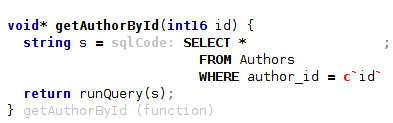
\includegraphics[width=0.50\textwidth]{screens/minisql_embedded.png}
	\caption{Embedding SQL code into C code and viceversa}
	\label{fig:sqlembedding}
\end{figure}

To demonstrate the flexibility of this approach we have also embedded our MiniSQL into the BaseLanguage, which is basically an implementation of Java in MPS. You can see it in \ref{fig:sqlembeddingjava}. Two separate extensions permit to embed the same language into different hosts (C and Java). For further explanations on this approach refer to \cite{Tomassetti2013}.

\begin{figure}[p]
	\centering
	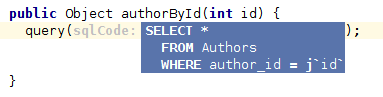
\includegraphics[width=0.50\textwidth]{screens/minisql_embedded_java.png}
	\caption{Embedding SQL code into Java code and viceversa}
	\label{fig:sqlembeddingjava}
\end{figure}

\subsubsection{Extension composition: combine independently developed extensions}
\label{evr:langcomp}

The mbeddr project contains many examples of language composition. Different extensions have been developed during the years, not necessarily from the exact same persons or in the context of the same project. However all of these extensions can be combined and used together.

A very interesting example is the Documentation language which permits to add references to other portions of code or to embed specificy contructs into the documentation.

In the example in \ref{fig:extensioncomposition} we can see a Documentation construct containing a table. The tables extensions have been developed separately, in a completely agnostic way, so that it could be reused in very different contexts. In this case it contains expressions from mbeddr language (C). So effectively three different extensions are combined in one single example.

\begin{figure}[p]
	\centering
	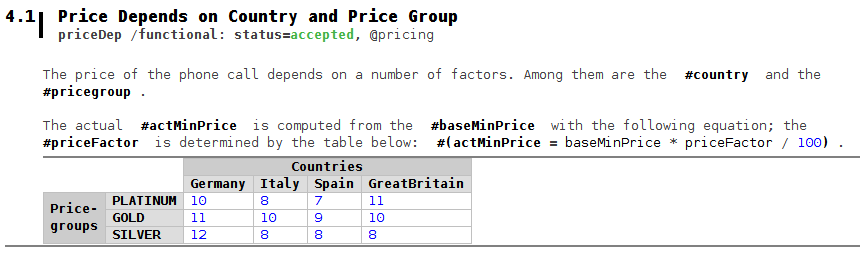
\includegraphics[width=0.50\textwidth]{screens/extension_composition.png}
	\caption{Combining tables, C expressions and the documentation language}
	\label{fig:extensioncomposition}
\end{figure}

\subsubsection{Beyond grammar restrictions: disallow constructs in certain scopes, without modeling this in the (abstract) syntax}
\label{evr:beyondgrammar}

MPS offers several mechanisms to limit where a certain construct can be used. In this respect it is not limited to the abstract syntax definition, but further logic can be added to additionally constraints the concepts usable in a given scope.

For example, every \emph{AssertStatement} is technically an mbeddr \emph{Statement}, from the point of the abstract syntax. However, an additional rule has been defined to restricted all constructs marked as \emph{IRestrictToTests} to be used exclusively in tests or tests related helper functions. This rule is visible in \ref{fig:restrictedtotest}.

\begin{figure}[p]
	\centering
	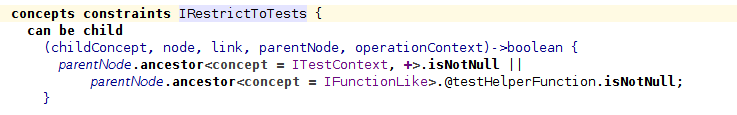
\includegraphics[width=0.50\textwidth]{screens/restricted_to_test.png}
	\caption{Rule which constraints the usage of certain constructs to tests}
	\label{fig:restrictedtotest}
\end{figure}

\subsubsection{Syntax migration: support migrating programs when concrete syntax changes}
\label{evr:synmigr}

\comment{TODO: to be written after the examples are provided}

\subsubsection{Structure migration: support migrating programs when abstract syntax changes}
\label{evr:structmigr}

\comment{TODO: to be written after the examples are provided}

\subsection{Variants}

The three first points we have seens (\ref{evr:langext}, \ref{evr:langembed}, and \ref{evr:langcomp}) have been solved through simple extension techniques. We do not see any obvious alternative for such cases. About combining independently defined extensions (\ref{evr:langcomp}) we can consider all the projects using the mbeddr platform as examples of this technique.

Regarding the grammar restrictions (\ref{evr:beyondgrammar}), we implemented it specifiying that certain rules can have as ancestors only certain nodes. Conversely we could have specified that certain rules could not contain specific descendants instead.

\subsection{Usability}

From the point of view of usability \ref{evr:langext}, \ref{evr:langembed}, and \ref{evr:langcomp} do not pose any issue. We simply used the mechanism of language extensions to add additional constructs to existing language. In one case we had done that for the specific goal to embed another language, while in the other cases we did not. In all cases the new constructs can be used exactly as the existing ones, so the new constructs are as usable as the previous ones with no different interactions required to the users.

The grammar restriction presented in \ref{evr:beyondgrammar} does not pose any usability issue neither. The whole mechanism is transparent to the user: elements which cannot be used in a certain context are not offered by the auto-completion mechanism and there is no immediate way to use them when they are not supposed to be used.

Migrations are typically performed through wizard dialogs. Those migrations are proposed to the user when MPS is started or the user can trigger them manually.

\subsection{Impact}

Language composition does not require to change existing elements.

\subsection{Composability}

Language composition is well supported in MPS. It is very natural and it does not require any particular technique. The only possible issues could be caused by semantic conflicts: supposed an expression language defines only statically evaluable expressions such literals and basic mathematical expressions. Suppose a first extension is based on this consideration and add the possibility to display the result of such expressions. Now, if a second extension would introduce non-statically evaluable expressions, the two extensions could not play well together. This problem could be avoidable by planning for extensibility in the original language: for example we could have required each Expression concept to declare if it was statically evaluable or not. All the expressions of the original language would have declared themselves to be statically evaluable, while the Expressions from the first extension would have not. The extensions calculating result values could have used the method to verify that all Expressions for which it wanted to calculate a value were indeed statically evaluable and trigger an error when not-statically evaluable expressions were used in the wrong context. In this way the two extensions would have played nice without being aware of each other.

\subsection{Limitations}

No particular limitations come to mind.

The only limitation we see is with migrations, because they are not reversible. This is an issue when different members of a team want to use different versions of MPS because each version comes with specific versions of the BaseLanguage: when a project is open with a new version migrations have to be performed and these migrations make the project incompatible with previous versions. Effectively this forces everyone to use the same version of the language workbench.

\subsection{Uses and examples}

Language extensibility and composition are used extensively in the two well-known MPS language families: the BaseLanguage and mbeddr. The BaseLanguage defines a core language and a set of independent extensions, mbeddr does the same.

\subsection{Effort (best-effort)}

The estimated effort for the different points is:

\begin{itemize}
	\item Language extension: XXX minutes
	\item Language embedding: 10 minutes
	\item Extension composition:
	\item Beyong grammar restrictions:
	\item Syntax migration:
	\item Structure migration:
\end{itemize}

For \emph{Language embedding} we calculate only the time for creating the concepts wrapping constructs of one language to be used in the other one (SQL into C and C into SQL). This time considers the definitions of the concepts, the editors, the typesystem rules and the code generators.

\subsection{Other comments}

\comment{Any idea?}

\subsection{Artifact}

\comment{TODO understand what should we write in this section}

%%%%%%%%%%%%%%%%%%%%%%%%%%%%%%%%%%%%%%%%%%%%%%%%%%%%%%%%%%%%%%%%%%%%%%%%%%%%%%%
%
% Editing Section
%
%%%%%%%%%%%%%%%%%%%%%%%%%%%%%%%%%%%%%%%%%%%%%%%%%%%%%%%%%%%%%%%%%%%%%%%%%%%%%%%

\section{Addressing the Editing Problem}

\subsection{Assumptions}

\subsection{Implementation}

\subsubsection{Editing incomplete programs: support for syntactically malformed programs}
\subsubsection{Referencing missing items: support referencing items that have not been defined}
\subsubsection{Structure agnostic copy-paste: copy-paste works across syntax boundaries}
\subsubsection{Restructuring: changing syntactic structure without typing the complete expression again.}
\subsubsection{Language demarcation: show how a combination multiple languages in one program are disambiguated}
\subsubsection{Delayed decisions: show when the syntactic category of an expression is determined}
\subsubsection{End-user defined formatting: show if and how user can change the visual appearance of the program}
\subsubsection{Specification of default formatting: support for pretty printing}
\subsubsection{Formatting preservation: how is formatting preserved when the code is automatically restructured}

\subsection{Variants}

\subsection{Usability}

\subsection{Impact}

\subsection{Composability}

\subsection{Limitations}

\subsection{Uses and examples}

\subsection{Effort (best-effort)}

\subsection{Other comments}

\subsection{Artifact}

%%%%%%%%%%%%%%%%%%%%%%%%%%%%%%%%%%%%%%%%%%%%%%%%%%%%%%%%%%%%%%%%%%%%%%%%%%%%%%%
%
% Conclusions
%
%%%%%%%%%%%%%%%%%%%%%%%%%%%%%%%%%%%%%%%%%%%%%%%%%%%%%%%%%%%%%%%%%%%%%%%%%%%%%%%

\section{Conclusions}

The JetBrains MetaProgramming System has significantly evolved during the years. Nowadays it is a powerful and flexible tool that can be used to address most of the Language Engineering challenges that have been brought forward in the LWC 2016.

\textbf{Notation}
\textbf{Evolution and Reuse}
\textbf{Editing}

%% We are using the command `bibtex' from within the directory `build', thus we need
%% to go back from this directory and look for the bibliography file.
\bibliographystyle{plain}
\bibliography{../LWC2016}

\end{document}
